\chapter{Implementation}\label{chap:implementation}
\todo{Jeg har ennå ikke presentert randbetingelser. Burde de inn i diskretisering eller i teorien?}We have now looked at the theoretical aspects of the level set method and constructed velocity models under the objective of approximating a curve with minimal curvature to a set of sampled points. Nothing is yet mentioned about the solution strategy and practical aspects. This chapter will answer questions concerning the technical implementation, the overall strategy chosen in this thesis, and possible pitfalls and approaches to overcome them. The entire code base for the implementation is written in Python. However, most of this chapter explains logic and algorithms which can be adapted to any preferred language.

More concrete, we will discuss spatial and temporal discretization techniques, suitable algorithms for producing the distance function and sign function, and how to prevent steep gradients from forming through a re-initialization procedure. We will first go into all aspects of the program separately and later put it all together and provide an overview of the main program.

Before moving on to the implementational details, we remind ourselves of the three models presented: the three partial differential equations we want our implementation to solve numerically.

\begin{alignat}{2}
    u_t &= |\nabla u|\,[\alpha\sigma(\mathbf{x}, t) d(\mathbf{x}; \pointsetm) + (1-\alpha) \kappa(u)], &\alpha \in \realspacem \label{eq:m1-imp}\\
    u_t &= |\nabla u|\, \bigg[\alpha \frac{ \sigma(\mathbf{x}, t)}{\beta d(\mathbf{x})+\delta} + (1-\alpha)\kappa (u) \bigg], &\alpha, \beta, \delta \in \realspacem \label{eq:m2-imp}\\
    u_t &= |\nabla u|\, \bigg[ \frac{\alpha \sigma(\mathbf{x}, t)}{\pi/2} \tan^{-1}\bigg(\frac{1}{\beta \distanceVm}\bigg) + (1-\alpha)\kappa (u) \bigg], \, &\alpha, \beta \in \realspacem \label{eq:m3-imp}
\end{alignat}

We begin with some notation concerning the discretization of the domain, \domain, and properties of the discretized problem. There are several ways to discretize the domain, and when efficiency is essential, adaptive mesh strategies or local methods can be of use. However, the focus for this project was more about investigating the behaviors of the proposed models, and the efficiency of the implementation was secondary. We thus chose a straightforward rectangular discretization.

All the sets of sampled points, \pointset, used in the following results have been fabricated data, and thus for simplicity, the domain, \domain, had been defined as $\domainm = [-1, 1]\times [-1, 1]$. The grid resolution is measured by the parameters $N_x$ and $N_y$ which is the number of nodes in respectively $x$- and $y$- direction. The corresponding grid size is then $h_x = 2/(N_x-1)$ and $h_y = 2/(N_y-1)$. 

We use the numbering of grid nodes as the convention for the Python package nympy's two-dimensional arrays. A grid point $(y_i, x_j)$ is positioned in the $i$th row counted from the bottom and $j$th column counted from the left. We have used numpy's \texttt{meshgrid} to produce the grid, which will be represented by the matrix $X$ containing both $x$- and $y$-coordinates. A grid node $(y_i, x_j)$ can thus also be represented as $X_{i, j}$. Note that this is a simplification of the \texttt{meshgrid} variables which saves the $x$- and $y$-coordinates in separate matrices $X$ and $Y$. \todo{Gå gjennom alle i og j for å sjekk at alt er riktig.}

\clearpage


\section{Temporal and Spatial Discretization} \label{sec:discretization}
This section will go through the discretization of the differential operators in the PDEs \eqref{eq:m1-imp} -- \eqref{eq:m2-imp}. This section will be rather short, as all spatial derivatives are discretized using central differences and the temporal discretization is the forward/explicit Euler method. 

Generally, we can express all models as 
\begin{equation*}
    u_t = |\nabla u| \, (\alpha f_p(\mathbf{x}) + (1-\alpha) \kappa(u)),
\end{equation*}
where $p=1, 2, 3$, and $f_p$ is the distance dependent velocity for model $p$. Expanding all terms and using \eqref{eq:curvature-u} in order to explicitly view all differential operators, this can be written as
\begin{equation}
    u_t = \alpha\, (u_x^2+u_y^2)^{1/2} f_p(\mathbf{x}) + (1-\alpha)\, \frac{u_{xx} u_y^2- 2u_{xy}u_xu_y + u_{yy}u_x^2}{(u_x^2+u_y^2)^{1/2}}.
    \label{eq:general-model-operators}
\end{equation}
We see from \eqref{eq:general-model-operators} that it is easy to switch between the different models by changing $f_p$.

From now on, when we discuss the discretization of the higher dimensional level set function, we will denote it as $U_{i, j}^{n} = u(x_j, y_i, t_n)$. 






%%%%%%%%%%%%%%%%%%%%%%%%%%%%%%%%%%%%%%



\section{Distance Functions} \label{sec:imp-dist}
In this setting, we use two types of distance functions, the signed and unsigned. We see from \eqref{eq:m1-imp} -- \eqref{eq:m3-imp} that the unsigned distance function to the point set, \pointset, is needed in in the velocity function for all models. In addition, as we discussed in \secref{sec:distance-function} that the signed distance function is a natural choice of level set function, \uxt, which is now the discretized $U^n(X_{i, j})$. We thus need algorithms to produce both types of distance functions on our discretized domain. We begin with the unsigned distance function.

First, note that numerically solving \eqref{eq:unsigned-distance-function} and \eqref{eq:unsigned-distance-function-curve}, which are the distance functions to respectively a set of points and a curve, reduces to the same problem. The discretized curve is only a set of coordinates where the curve crosses the grid lines. Thus, the following algorithm is a numerical approximation to both \eqref{eq:unsigned-distance-function} and \eqref{eq:unsigned-distance-function-curve}.

The straightforward approach to solve any minimization problem is to go through every alternative value and choose the minimal value. Interpreted for this problem---for all grid points $X_{i, j}$, make an array of the distance to all points in the point set and return the minimum of these.

\begin{algorithm}[H]
\SetAlgoLined
$d(\mathbf{x}; \pointsetm)=\texttt{zeros}(N,M)$\;

 \For{$i\gets0$ \KwTo $N_y$}{
    \For{$j\gets0$ \KwTo $N_x$}{
    $d$[i, j] = 0 \;
    \ForEach{$v \in \pointsetm$}{
    \If{$\|X[i, j] - v\|< d[i, j]$}{$d[i, j]=\|X[i, j] - v\|$\;}
    }
    }
    }
\KwResult{$d(\mathbf{x}; \pointsetm)$}
 \caption{Direct approach for distance functions}
 \label{alg:direct-distance}
\end{algorithm}

We see that \algref{alg:direct-distance} has a quadratic complexity with respect to the grid size and also increasingly dependent on the size of the sample points \pointset. For each grid point, the distance to all sample points must be calculated before choosing the minimum. The complexity is thus $\mathcal{O}(N_x\times N_y \times V)$ for $V=\texttt{size}(\pointsetm)$. Furthermore, when Algorithm \ref{alg:direct-distance} is applied to a discretized curve, the resolution increases with $N_x$ and $N_y$ so the size of the coordinate set defining the curve increases. In that case, the size of the point set will also increase with $N_x$ and $N_y$ and thus scale even worse.

As we just saw, the approach is very time-consuming for the implementation of distance functions to curves. We observed in the first implementation, which used Algorithm \ref{alg:direct-distance}, that this considerably slowed down the overall run time. For that reason, we were on the look for something else. The answer became the \textit{Fast Marching Method} derived and developed by Sethian in the $90$s, and a thorough introduction can be found in his book\cite{sethian1999level}.

\begin{comment}
The unsigned distance function is only used in the initialization to calculate \distanceV\ defined in \eqref{eq:unsigned-distance-function}, namely the distance to the point set, which is constant throughout the algorithm. The signed distance function, \signeddistance, on the other hand, is both used in the initialization to construct the initial higher dimensional curve and in the re-initialization procedure.

From \secref{sec:distance-function} we saw that finding the unsigned distance function to an object is really solving the minimization problem \eqref{eq:unsigned-distance-function}. We also saw that the signed distance function, \signeddistance, is only an unsigned distance, $d(\mathbf{x}, \curvem)$, where it is multiplied with a negative sign on the inside of the curve. In addition, in a discretized setting, the zero level set curve is also a set of points where $\uxtm=0$ and thus similar to $d(\mathbf{x}, \pointsetm)$.

For this reason, both the signed distance to the curve and the unsigned distance to the point set reduces to the same problem: solving \eqref{eq:unsigned-distance-function} for a set of points. Solving this equation is thus where we begin.

The most obvious way to solve the minimization problem \eqref{eq:unsigned-distance-function} is to approach it straight forwards as it is stated: for all grid points, go through all the sample points, find the closest one and return the distance. 
\end{comment}






\subsection{The Fast Marching Method}
The Fast Marching Method is a standard method for solving an equation called \textit{the Eikonal equation}. We will first show that the distance function is only a special case of the Eikonal equation and then present the idea behind the Fast Marching Method. 

\begin{definition}[The Eikonal Equation]
Assume that we are tracking an expanding front $\Gamma(t)$, expanding with a velocity $v_n(\mathbf{x}, t)$ from an initial curve $\Gamma_0$. The time of arrival, $T(\mathbf{x})$ is the time the front crosses the point $\mathbf{x}$. This function $T(\mathbf{x})$ can be found by solving the Eikonal equation \cite{sethian1999level}
\begin{equation}
    |\nabla T(\mathbf{x})| = \frac{1}{v_n(\mathbf{x}, t)}. 
    \label{eq:eikonal-eq}
\end{equation}
\end{definition}
Recalling $|\nabla d(\mathbf{x}, \cdot) | = 1$, we immediately see that the distance function must satisfy \eqref{eq:eikonal-eq} for a velocity $v_n=1$. It is in fact obvious that the travel time and distance traveled is identical when $v_n=1$ by the physical fact that $\texttt{time=distance/speed}$. From now on, we thus replace the time of arrival $T$ to the distance $d(\mathbf{x}, \Gamma)$ when $v_n=1$.

The time of arrival at a grid point $X_{i, j}$ is uniquely defined by the time of arrival of the neighboring grid points where the front has already crossed. Thus information spreads outwards, and upwind schemes are appropriate to use. The direction of the upwinding is decided by which direction the time increases. The resulting upwind scheme \cite{sethian1999level} for solving \eqref{eq:eikonal-eq} for a speed of propagation $v_n = 1$ is

\begin{equation}
\begin{split}
        \big[ &\max (D^{-x}_{j, i} d(\mathbf{x}, \Gamma), 0)^2 + \min (D^{+x}_{j, i} d(\mathbf{x}, \Gamma), 0)^2  \\
    + &\max (D^{-y}_{j, i} d(\mathbf{x}, \Gamma), 0)^2 + \min (D^{+y}_{j, i} d(\mathbf{x}, \Gamma), 0)^2 \big] = 1
    \end{split}
    \label{eq:upwind}
\end{equation}

The operators $D^{-x}_{j, i} d(\mathbf{x}, \Gamma)$ and $D^{+x}_{j, i} d(\mathbf{x}, \Gamma)$ is the corresponding backward and forward difference operators
\begin{equation*}
    D^{-x}_{j, i} d(\mathbf{x}, \Gamma) = \frac{d(X_{j, i})- d(X_{j, i-1})}{h_x}, \qquad D^{+x}_{j, i} d(\mathbf{x}, \Gamma) = \frac{d(X_{j, i+1})- d(X_{j, i})}{h_x}.
\end{equation*}
We see that \eqref{eq:upwind} automatically chooses the direction where the derivative increases and thus ensures that information flows from small to big distances, meaning from the curve and outwards.

The overall strategy is to mark all grid points with known values in a list $K$, and calculate the values in their neighboring points using the upwind scheme \eqref{eq:upwind} and store them in a data structure $T$. The list $K$ stands for \textit{known} and $T$ for \textit{trial} which must contain both the grid point and trial value. 

Since all information travels from smaller to higher values, the smallest value of $T$ must be independent of all the other points in $T$, and thus it must have the correct value. Hence, the strategy is to continually move the smallest point in $T$ to $K$ and recalculate its neighbors. We summarize this in the algorithm below.

\begin{algorithm}[H]
\SetAlgoLined
$d(X; \Gamma)=\texttt{zeros}(N,M)$\;
$T = \texttt{Array\{ (i, j) : 0\}} \qquad$ for $(i, j) \in \Gamma$\; 
$K = \texttt{Array \{\}}$

\While{$T\neq \{ \}$}{
    $(i, j) = \texttt{argmin}(T)$ \;
    $u_d(i, j) = T(i, j)$ \;
    $K \pluseq (i, j)$ \;
    $T \minuseq (i, j)$ \;
    $N = \texttt{neighbors}(i, j) \notin K$\;
    \For{$(p, q) \in N$}{
        $T \pluseq (p, q) : (\texttt{solve \eqref{eq:upwind}})$
    }
}
\KwResult{$d(\mathbf{x}; \Gamma)$}
 \caption{The Fast Marching Method for Distance Functions}
 \label{alg:idea-fmm}
\end{algorithm}

For a rectangular grid, each grid point can at most be recalculated four times because it only has four neighbors. Thus it will have a worst-case complexity bounded by $\mathcal{O}(4 (N\times M))$, which can be significantly smaller than the complexity of Algorithm \ref{alg:direct-distance}. The fast marching method becomes increasingly superior for large point sets or equivalently increasing grid resolution when calculating the distance function to curves.

There exists a python extension module named \texttt{scikit-fmm} which implements the Fast Marching Method. It is open-source, and both the code and documentation can be found on GitHub \footnote{\texttt{https://github.com/scikit-fmm/scikit-fmm}}


%\subsection{The Fast Marching Method}
The idea behind the Fast Marching Method is to utilize that the Eikonal equation is a boundary value problem, meaning that all the information travels in one direction at all times -- from the curve and outwards. Thus a solution can be obtained only from upwind values. 

\todo{Fyll inn upwind skjema for å regne ut Eikonal eq i punkt (i, j)}

The over all strategy is then to mark all grid points with known values in a list $K$, and calculate the values in their neighboring points using the upwind scheme \textbf{(??)} and store them in a data structure $T$, which stands for \textit{trial}, containing both the grid point and trial value. The smallest value in $T$ must have correct value, because all information flows from smaller to greater values and thus it has to be independent of all other points in $T$ \cite{sethian1999level}.

This more algorithmically formulated as \\
\begin{algorithm}[H]
\SetAlgoLined
$u_d(\mathbf{x}; \Gamma)=\texttt{zeros}(N,M)$\;
$T = \texttt{Array\{ (i, j) : 0\}} \qquad$ for $(i, j) \in \Gamma$\; 
$K = \texttt{Array \{\}}$

\KwResult{$u_d(\mathbf{x}; \Gamma)$}

\While{$T\neq \{ \}$}{
    $(i, j) = \texttt{argmin}(T)$ \;
    $u_d(i, j) = T(i, j)$ \;
    $K += (i, j)$ \;
    $T -= (i, j)$ \;
    $N = \texttt{neighbors}(i, j) \notin K$\;
    \For{$(p, q) \in N$}{
        $T += (p, q) : (\texttt{solve}(\textit{Eikonal equation w/upwind scheme}))$
    }
}
 \caption{The Fast Marching Method}
 \label{alg:idea-fmm}
\end{algorithm}

For a rectangular grid, each grid point can at most be the neighbor of four other points before being redefined to \textit{known}. Thus it will have a worst case complexity bounded by $\mathcal{O}(4 (N\times M))$, which can be significantly smaller than the complexity of Algorithm \ref{alg:direct-distance} for large point sets.

Note that the Fast Marching Method can be used to produce both signed and unsigned distance functions. The speed $F$ has direction normally outwards of the curve or known points, and by setting $F=-1$ on the inside of the curve yields a signed distance function.

There exists a Python package named $\texttt{scikit-fmm}$ which implements the Fast Marching Method. The function $\texttt{distance}()$ will produce the signed distance function, but a pure distance function can be produced with the built-in function $\texttt{travel\_time} ()$ using a velocity $F=1$ outside and $F=-1$ inside the curve\footnote{\texttt{https://pythonhosted.org/scikit-fmm/}}.

Both Algorithm \ref{alg:direct-distance} and Algorithm \ref{alg:idea-fmm} could thus be used in the Level set Algorithm

This Algorithm can be applied in the initialization of the solver, when calculating $d(\textbf{x})$ and $u_0(\Gamma)$ and also when re-initializing. 



\clearpage
\section{Sign Function, \texorpdfstring{$\sigma (\mathbf{x}, t)$}{sigma}} \label{sec:signfunction}
The purpose of the sign function, $\sigma(\mathbf{x}, t)$ is explained in \chapref{chap:modeling}---to pull the curve towards the point set. Since positive normal-velocity is defined inwards, the sign should be positive when the curve is outside of the point set and oppositely negative when it is inside the point set. The sign function is defined in \eqref{eq:sigma-def}, but we repeat it in its discretized version.
\begin{equation}
    \sigma(X_{i, j}, t) = \texttt{sgn}((u(\mathbf{v}_r, t))), \quad \mathbf{v}_r = \texttt{argmin}(\|X_{i, j}- \mathbf{v}\|_2\, \forall \, v\in \pointsetm). 
    \label{eq:sigma-function}
\end{equation}
We see that calculating $\sigma(X_{i, j}, t)$ numerically, in practice consists of two problems: solving a minimization problem to find the closes point in \pointset\ and calculating the sign of the higher dimensional level set function $U^n(X_{i, j})$ at the closest point. The latter may seem easy, but since the discretized $U_{i, j}^n$ is known only at the nodes on the grid, and $\mathbf{v}_r \in \pointsetm$ may be located independently of the grid, the value on $\mathbf{v}_r$ may not be given directly. The values of the higher dimensional function at the sampled points thus have to be interpolated from the neighboring grid points in general except for particular cases where the sample points are located on a node.

We use bilinear interpolation to approximate the value of $U^n(\mathbf{v}_r)$ from the discretized values $U_{i, j}^n$. We can approximate the higher dimensional function $u(x, y, t)$ for a fixed $t=t^*$ on a grid cell $[x_i, x_{i+1}]\times [y_j, y_{j+1}]$ using the following formula \cite{Press2007Numerical}
\begin{equation}
\begin{split}
    &u(x, y) = \\
    &\frac{1}{(x_{i+1}-x_i)(y_{i+1}- y_i)} \begin{bmatrix} x_{i+1}- x & x - x_i \end{bmatrix} \begin{bmatrix} U_{i, j} & U_{i, j+1} \\ U_{i+1, j} & U_{i+1, j+1} \end{bmatrix} \begin{bmatrix} y_{i+1}-y \\ y-y_i \end{bmatrix}
\end{split}
\label{eq:bilinear-interpolation}
\end{equation}

This equation requires that the cell containing $\mathbf{v}_r$ is known. We will soon see that the closest point is easy to obtain directly in the implemented data structure, but this is not the case for the other three nodes. Hence, we will now present an algorithm that finds the three last cell nodes from the closest grid node and then approximates the higher dimensional function in the point $\mathbf{v}_r \in \pointsetm$. The procedure is to first locate the relative position of the point $\mathbf{v}_r$ compared to the closest grid point to find out in which of the four neighboring cells it is contained. Then use these four grid points to solve \eqref{alg:bilinear-interpolation} for $x$ and $y$ being the coordinates of $\mathbf{v}_r$.
\clearpage

\begin{algorithm}[H]
\SetAlgoLined
$i_1, j_1 = \texttt{closestPoint}(\mathbf{v}_r)$ \tcp*{Grid numbers for closest point}
$x_1, y_1 = X[i_1, j_1]$  \tcp*{Grid values for closest point}
$x_v, y_v = \mathbf{v}_r$  \tcp*{Coordinates of $\mathbf{v}_r$} 
$d_1 = x_v-x_1$ \;
$d_2 = y_v - y_1$ \;
$x_2 = x_1$\;
$y_2 = y_1$ \;
\tcc{Check where $\mathbf{v}_r$ is located relatively to the closest point}
\If{$d_1 > 0$}{
    $i_2 = i_1 + 1$ \;
}
\ElseIf{$d_1<0$}{
    $i_2 = i_1 - 1$ \;
}
\If{$d_2 > 0$}{
    $j_2 = j_1 + 1$ \;
}
\ElseIf{$d_2<0$}{
    $j_2 = j_1 - 1$ \;
}
\tcc{Define the four points needed for bilinear interpolation}
$U_1 = U[j_1, i_1]$ \;
$U_2 = U_[j_1, i_2]$ \;
$U_3 = U_[j_2, i_1]$ \;
$U_4 = U_[j_2, i_2]$ \;

\tcc{Solve \eqref{eq:bilinear-interpolation}}
$\mathbf{b}_1 = [h_x - \texttt{abs}(d_1), \texttt{abs}(d_1)]$ \;
$A = [[U_1, U_2], [U_3, U_4]]$ \;
$\mathbf{b}_2 = [h_y - \texttt{abs}(d_2), \texttt{abs}(d_2)]$ \;

$u(x_v, y_v) = \frac{1}{h_x h_y} \mathbf{b}_1 A \,\textbf{b}_2^T$ \;
\KwResult{$u(x_v, y_v)$}

 \caption{Bilinear Interpolation from Closest Grid Point}
 \label{alg:bilinear-interpolation}
\end{algorithm}

\clearpage
\section{Re-initialization} \label{sec:reinitialization}
\todo{Burde jeg bruke U over alt?}We discussed in the theoretical section on level set methods that $|\nabla u|$ scales the change in \uxt\ needed to move the curve with the given speed $v_n$. The velocity functions defined for our models are all dependent on the curvature and distance, which is not the same for all level curves. The result is that they move with different speeds, and the shape of \uxt\ loses the property that $|\nabla u|=1$ everywhere. 

For the implemented discretization techniques, steep gradients are a problem in themselves because there could be formed oscillations near the steep regions, which can ruin the solution if they grow big enough. Also, it has been shown, for example by D. Peng et al. \cite{Fast-PDE} that the evolution of the curve may be unstable if the gradient is too steep or flat. The procedure of re-initializing will keep the gradient from deviating much from $|\nabla U|=1$ by restarting the procedure but not reset the time. 

What this means in practice is that the zero level set $\Gamma^n$ of the last temporal solution $U^{n}$ will form the starting curve of a new level set problem. Thus, we form a signed distance function $\tilde{U}^n$ from $\Gamma^n$ and then $\tilde{U}^n$ is used as the higher dimensional level set function.

The signed distance function can be formed in two ways. The first one is using the straight forward approach for calculating a distance function from Algorithm \ref{alg:direct-distance} and multiply with the sign of the old level set function $U^n$. This works because $\Gamma^n$ is the zero level set of both $U^n$ and $\tilde{U}^n$. This means solving
\begin{equation}
    \tilde{U}^{n} = d(\mathbf{x}; \Gamma^{n})\cdot \texttt{sign}(U^{n}).
\end{equation}
As described in \secref{sec:imp-dist}, Algorithm \ref{alg:direct-distance} is time consuming and especially poor suited for computing distances to a discretized curve. Thus, the faster approach, which is the one implemented in the code base for this thesis, is the Fast Marching Method.

Using the \texttt{scikit.fmm} package in Python is especially easy, as it is perfectly compatible with level set functions. It takes a higher dimensional function as input, together with the grid size, and returns a signed distance to the curve using \texttt{skfmm.distance()}.


\section{Updating the sign function, \texorpdfstring{$\sigma (\mathbf{x}, t)$}{sigma}} \label{sec:data-struc}
Whether\todo{Se på denne overskrifta. Det funker ikke helt} or not the sign function should be updated is given by the sign of $U^n$ at the points $\mathbf{v}\in\pointsetm$. Thus, we have chosen to define the points in the point set as a class object where the sign is a state variable. If the state is changed, it triggers an update process for the sign function. Going back to the definition of $\sigma(\mathbf{x}, t)$, we can see that since the points $\mathbf{v}\in\pointsetm$ never move, there is no need to calculate the $\mathbf{v}_r = \texttt{argmin}(\|\mathbf{x}-\mathbf{v}\| \, \forall \, \mathbf{v} \in \pointsetm)$ more than once. 

To cut down on computations, we store a list of objects $\{\mathbf{v}_r \, \forall \, \mathbf{v} \in \pointsetm\}$, where the point $\mathbf{v}_r$ stores the coordinate of the point, the sign of \uxt\ in that point, and what will be refered to as the cohort of $\mathbf{v}_r$. The cohort of $\mathbf{v}_r$ is a list of all the grid nodes $X_{i, j}$ that has $\mathbf{v}_r$ as the solution of $\mathbf{v}_r = \texttt{argmin}(\|X_{i, j}-\mathbf{v}\| \, \forall \, \mathbf{v} \in \pointsetm)$. Thus, at every iteration, when we check for updates in $\sigma(\mathbf{x}, t)$, we only need to go through the points in the point set, estimate the sign of \uxt\ at the sample points and update its cohort in stead of recalculating \eqref{eq:sigma-function} again.

This structure is also the reason why we stated in \secref{sec:signfunction} that it is easy to request the single closest grid point to a point $\mathbf{v}_r \in \pointsetm$, but not the four closest. Look at \figref{fig:grid-to-point} for reference. There we have two sample points where both have at least three grid points in their cohort. If there is more than one sample point inside each cell, each sample point could have down to zero grid points in their cohort. If a point $\mathbf{v}_r$ has zero grid points in its cohort, the sign of $\mathbf{v}_r$ does not matter, and we do not need to estimate the sign. Else, we have at least one, which means we can always use Algorithm \ref{alg:bilinear-interpolation}. If the sign of $u(\mathbf{v}_r, t)$ has changed, it is easy to update $\sigma$. It is done only by changing the sign of all grid points in the cohort of $\mathbf{v}_r$.

\begin{figure}
    \centering
    \begin{subfigure}[b]{0.2\linewidth}
        \centering
        \includegraphics[width=\linewidth]{figures/tikz-figures/points-cohort.tex}
        \caption{Cohort of two neighboring sample points}
        \label{fig:grid-to-point}
    \end{subfigure}
    ~
    \begin{subfigure}[b]{0.7\linewidth}
    \centering
        \includegraphics[width=\linewidth]{figures/Implementation/punktsett-område-4-cropped-1.jpg}
        \caption{Two different curves, $\Gamma_1$ and $\Gamma_2$. The areas are the cohorts of grid points for the three sample points.}
        \label{fig:pointset-with-area}
    \end{subfigure}
    \caption[The Cohort of a Point Set]{To the left we see how the grid points are assigned to their cohorts. To the right we see that for $\Gamma_1$ the sign function $\sigma$ must be positive for all grid points. For $\Gamma_2$ on the other hand, the sign function must be negative for all the points in the upper left region, that is the cohort of the upper left sample point.}
    \label{fig:datastruc-pointset}
\end{figure}
\todo{Fix (a) og placement i neste figur}
\begin{algorithm}[H]
\SetAlgoLined
\For{$v \in \pointsetm$}{
    $u(v) = \texttt{bilinear\_interpolation}(v.\texttt{closest\_point})$ \;
    \If{$u(v) \neq v.\texttt{sign}$}{
        $\sigma[v.\texttt{cohort}] \multeq -1$ \;
        $v.\texttt{sign} \multeq -1$ \;
    }
}

\KwResult{$\sigma(\mathbf{x}, t^{n})$}
 \caption{Updating the Sign Function}
 \label{alg:update-sigma}
\end{algorithm}
\section{The Main Algorithm} \label{sec:main-alg}
Now that we have explored the important parts of the code base, we will put it all together and present the structure of the main algorithm and how the small pieces fit together. We see in \figref{fig:flow-algorithm} a flow chart displaying the overall flow of the algorithm. 

\begin{figure}
    \centering
    \includegraphics[width=\linewidth]{figures/tikz-figures/Algorithm.tex}
    \caption[Algorithm - overview]{Caption}
    \label{fig:flow-algorithm}
\end{figure}

In the $\texttt{Initialization}$, we set up the grid, calculate the distance function \distanceV, set up the sample points with a corresponding initial sign and find their respective cohorts. To assign all grid points to a cohort, we loop through all grid points to find the closest sample point. This is easily combined with Algorithm \ref{alg:direct-distance}, and thus we do not use the Fast Marching Method in the initialization. This procedure is only done once, and thus, we tolerate that it is not as efficient. 

Moving on to the \textit{Time integration} in \figref{fig:flow-algorithm}, we remember that our time integrator is an Explicit Euler method which is a one-step method. We perform $s$ time integration steps, where at all steps, the sign function needs to be updated. After $s$ steps, the shape of the higher dimensional function may be deviating so much from a signed distance function that we reinitialize to obtain once more a $U^n$ that satisfies $\|\nabla U\|=1$.

Because $U^n$ is now exclusively decided by the zero level set curve, this is the perfect place to propose a stopping criterion to check for convergence. We have reached the stationary solution when the zero level set curve $\Gamma^n$ is equal to $\Gamma^{n-1}$ and when $U$ is a signed distance function, this corresponds to $U^n$ equal to $U^{n-1}$. Thus a stopping criterion could be to stop if 
\begin{equation}
    \|U^n - U^{n-s}\|_2 < \varepsilon,
    \label{eq:stopping-criterion}
\end{equation}
for some $\varepsilon>0$.

Note that, as we remember from the analysis of the circular examples for model 2 and model 3, what looked like a stationary solution, actually had a non-zero speed. However, because of the sign change at the radius of the point set, the curve stopped moving in the analytical streamline figures, see \figref{fig:total-streamline-inverse} and \figref{fig:total-streamline-arctan}. When we move with finite time steps, the non-zero speed will cause the curve to oscillate around the radius of the point set. This kind of behavior could result in a curve that looks stationary over time but never actually trigger the stopping criterion.

The value of $s$, meaning the number of time steps between reinitializations, could vary from problem to problem. It depends on how big the velocity of each level curve is and how big of a time step we use. A rule of thumb is to reinitialize too frequently rather than too seldom. The only drawback to reinitializing too often is that it slows down the total runtime.



%%%%%%%%%%%%%%%%%%%%%%%%%%%%%%%%%%%%%%%%%%%%%%%%%%%%%%
%\section{Updating the Sign Function}
The purpose of the sign function $\sigma(\mathbf{x}, t))$ is to pull the curve in the right direction. As stated, the sign function should be positive when the curve is outside the point set and negative if it is inside of the point set. This may seem like a simple task at first glance, but deciding whether or not the curve should move inwards or outwards is not simple at all.

We first present the strategy that is chosen in our implementation, namely pulling the curve towards its closest points. There is a clear reason behind our choice, but there certainly are drawbacks to the strategy as well, which we will shed light on during this discussion.

The information needed to pull the curve towards the closest point at all times is first of all what parts of space that are closest to which data points and then whether or not that data point is inside or outside of our curve. This is kind of the equivalent but opposite way of looking at the problem, namely whether or not the data points are inside or outside the curve. 


\begin{algorithm}[H]
\SetAlgoLined




\For{$\texttt{contour} \in \texttt{contour\_curves}$}{
    $\texttt{coords}_{t+1} = \texttt{contour}.\texttt{collections.get\_paths().vertices}$ \;
}
\If{$\texttt{shape}(\texttt{coords}_{t+1}) == \texttt{shape}(\texttt{coords}_{t})$}{
    \If{$\|\texttt{coords}_{t+1} - \texttt{coords}_t\|_2 \leq \epsilon$}{
    $\texttt{continue} = \texttt{False}$ \;
    }
}
\KwResult{$\sigma_{n+1}(X, Y)$}
 \caption{Updating $\sigma(\mathbf{x}, t)$}
\label{alg:update-sign}
\end{algorithm}



%%%%%%%%%%%%%%%%%%%%%%%%%%%%%%%%%%%%%%%%%%%%%%%%%%%%%%%%%%%%%%%%%%%
The distance function is local, meaning that it only knows the distance to the closest point and knows nothing about the global arrangement of points. This is the main reason why the sign function is chosen as it is. Remember that it is the distance function which provides the speed and the sign function that decides the direction of the distance-dependent velocity and it is most elegant that the speed and direction is constructed from the same information.

Although it is reasonable, it is not obvious, and there are several reasons why one could want something else. Say that you have noise in your data, and the most obvious curve to draw is one that does not go through any of the points, but passes somewhere in the middle. This kind of behavior would not be encouraged by such a local sign function. 


From the initialization, we saw that the starting curve was chosen to surround all the points in the point set, meaning that the sign function must be positive everywhere. For the behavior of the curve, this means that the distance term is contributing to the speed inwards -- towards the point set. In such cases, where the curve is outside the point set, the sign function has an obvious value. However this is maybe the only situation where this is obvious. 

Say you have noise in your data, and there is no obvious structure in the arrangement of the data points. Then it can be hard to determine whether or not anything is inside or outside of your data points. There could also be situations where the curve is inside and outside simultaneously, if for example again, there are noise and the curve lies somewhere in between data points.

By looking at the data set and the curve, it could be obv

\clearpage
%\section{Initialization}
The initialization of the algorithm mainly consists of the following parts: Setting up the grid, calculating $u(\mathbf{x}, 0)$ from the initial curve $\Gamma(0)$, calculating \distanceV\ and initializing the sign function $\sigma(\mathbf{x}, 0)$. 

For a rectangular grid with equidistant grid points, the construction is very simple and we will thus only discuss it briefly. In python the numpy package contains useful functions like $\texttt{linspace}(x_{\text{start}}, x_{\text{end}}, N)$ producing an array of equidistant points and $\texttt{meshgrid}(x, y)$ for producing a two dimensional grid spanned by the discretized $x$- and $y$-axis. 

The initialization of the higher dimensional function, $u$, consists of calculating a signed distance function to the initial curve, $\Gamma(0)$. Because the algorithm does not assume anything about the structure or the shape of the final curve, we use a function encircling our point set, \pointset. An additional advantage when using the circle as initial curve is that the signed distance is very easy to compute.

For an initial circle $\Gamma(0)$ with center in $\mathbf{c}$ the signed distance at a point $\mathbf{x}$ is given as
\begin{equation}
    d(\mathbf{x}, \Gamma(0)) = \sqrt{(\mathbf{x}-\mathbf{c})^T(\mathbf{x}-\mathbf{c})}-r_{\Gamma}.
    \label{eq:signed-distance-circle}
\end{equation}

The next step is calculating the distance function to the point set and initializing $\sigma(\mathbf{x}, 0)$. Since the initial curve is chosen to surround all points, the initial sign is automatically positive on the whole domain. Nevertheless, the data structure needed to update the function needs to be set up. 

\todo{Skriv om sigma i modellering før du forklarer mer}

\begin{algorithm}[H]
\SetAlgoLined
$\sigma = \texttt{ones}(N, M)$ \;
$V = \{\texttt{sample\_points}(\texttt{coordinates}=\{v\}, \texttt{closest\_points}=\{\})\}$ \;
$d = \texttt{zeros}(N, M)$



\For{$i\gets0$ \KwTo $N$}{
    \For{$j\gets0$ \KwTo $M$}{
        \tcc{Calculate closest point in point set and assign the grid point to that point}
        $d(i, j) = \{\|X(i, j)- v\|$ \textbf{for} $v\in \pointsetm$\}.\texttt{min}() \;
        $c_v= \{\|X(i, j)- v\|$ \textbf{for} $v\in \pointsetm$\}.\texttt{argmin}() \tcp*{The closest sample point}
        $V(c_v).\texttt{closest\_points} \pluseq X(i, j)$ \;
    }
}
\KwResult{$V$, $\sigma$, $d$}
 \caption{Initializing $\sigma(\mathbf{x})$ and $d(\mathbf{x};\pointsetm)$}
 \label{alg:sigma-dist}
\end{algorithm}


\begin{comment}
\begin{itemize}
    \item Setting up the grid 
    \item Initializing $\sigma(\mathbf{x}, 0)$
    \item Calculating \distanceV
    \item Initializing \uxt
\end{itemize}
\end{comment}

\clearpage
%\section{Time Integration and Spatial Discretization}
The time integration step is the part where we integrate our partial differential equation to evolve forward in time. In order to do so, we need a numerical ODE solver for the time integration and we need to discretize the spatial differential operators.

We begin with the discretization of the spatial operators. First note that we have shown in \secref{sec:levelset-methods} that the curvature $\kappa(u)$ in \eqref{eq:our-model-restated} can be written in terms of the spatial derivatives of $u$ as 
\begin{equation*}
    \kappa(u) = \frac{u_{xx} u_y^2- 2u_{xy}u_xu_y + u_{yy}u_x^2}{(u_x^2+u_y^2)^{3/2}}.
\end{equation*}
Also note that the absolute value of the gradient of u from \eqref{eq:our-model-restated} is in two dimensions written as 
\begin{equation*}
    |\nabla u| = (u_x^2+u_y^2)^{1/2}.
\end{equation*}
Because our distance dependent function $f(\distanceVm)$ is purely a function of the distance function and not dependent of $u$, we can write the PDE for the general model \eqref{eq:our-model-restated} as

\begin{equation}
    u_t = \alpha\, (u_x^2+u_y^2)^{1/2} f(\distanceVm) + (1-\alpha)\, \frac{u_{xx} u_y^2- 2u_{xy}u_xu_y + u_{yy}u_x^2}{(u_x^2+u_y^2)^{1/2}}.
\end{equation}

The curvature term makes the equation parabolic and thus a straight forward approach is to discretize the derivatives using a central difference approximation. These can be found in the Appendix \todo{Legg inn og referer}. 

Now, what is left is solving the resulting ODE with respect to time. In our implementation, we have used a simple forward Euler scheme which means that the time steps bounded by the CFL-condition can be as small as 


\begin{equation}
    \Delta t \leq \frac{1}{2} h^2
\end{equation}
\todo{Dette kan ikke stå sånn. Enten må man gjøre mere analyse, eller gi en vagere advarsel om /stabilitet.}

\clearpage
%\section{A Stopping Criterion}
It has already been mentioned in \chapref{chap:modeling}, that the PDE only has a local stationary solution at the curve. Thus, a stopping criterion can not be dependent on the global shape of the higher dimensional function, \uxt, but only its zero level curve \curve. 

Because the curve is only tracked implicitly, we do not know the localization of the curve directly on the grid, but it needs to be approximated from the values of \uxt on the grid points. In python, there is a function in the matplotlib package called $\texttt{contour}()$ which given the grid and grid values of $U$ and the value for the desired level curve(s) returns an object of contour sets which also contains a list of coordinates where the level curves crosses the grid lines.

Note that this can also be implemented manually by finding all pairs of grid points where the higher dimensional function changes sign and do a linear interpolation to find the approximate coordinate of crossing. 

Given a list of coordinates where the zero level curve crosses the grid lines, a stopping criterion can be implemented by comparing the most recent zero level curve list with the one from the previous time step. A first check can be to compare the size of the lists, and if it does, then compute for example the Eucledian distance between them. 

\begin{algorithm}[H]
\SetAlgoLined
\texttt{import matplotlib.pyplot as plt} \;
$\texttt{continue} = \texttt{True}$ \;
$\texttt{coords}_t = \texttt{Array} \{(x_i, y_i) \text{ for } (x, y)\in \Gamma_t \}$ \;



$\texttt{contour\_curves} = \texttt{plt.contour}(X, Y, U_t, levels=[0])$ \;

\For{$\texttt{contour} \in \texttt{contour\_curves}$}{
    $\texttt{coords}_{t+1} = \texttt{contour}.\texttt{collections.get\_paths().vertices}$ \;
}
\If{$\texttt{shape}(\texttt{coords}_{t+1}) == \texttt{shape}(\texttt{coords}_{t})$}{
    \If{$\|\texttt{coords}_{t+1} - \texttt{coords}_t\|_2 \leq \epsilon$}{
    $\texttt{continue} = \texttt{False}$ \;
    }
}
\KwResult{\texttt{continue}}
 \caption{Stopping criterion}
\label{alg:stopping-criterion}
\end{algorithm}

\clearpage




%\section{Space Discretization} \todo{Begynn på nytt på dette..}
For the two-dimensional case, we rewrite the right hand side of \eqref{eq:model1-pde} in order to see if it can be simplified. 

\begin{proposition}\label{prop:simplification-equation}
In two spatial dimensions, \eqref{eq:pde-eq1-num} can be written as
\begin{equation}
    u_t = (1-\alpha)\, \frac{u_x^2 u_{yy} - 2 u_{xy} u_x u_y + u_y^2u_{xx}}{u_x^2 + u_y^2} + (u_x^2 + u_y^2)^{\frac{1}{2}}\alpha \sigma d
    \label{eq:pde-written-out}
\end{equation}
\end{proposition}

\begin{proof}
\begin{equation}\label{eq:proof-writeout}
    \begin{aligned}
        u_t &= |\nabla u| \bigg[(1-\alpha)\,(\nabla \cdot \bigg(\frac{\nabla u}{|\nabla u|}\bigg) + \alpha d \bigg] \\ &= |\nabla u|\,(1-\alpha)\,\bigg( \nabla \cdot \bigg(\frac{\nabla u}{|\nabla u|}\bigg) \bigg) + |\nabla u| \alpha d
    \end{aligned}
\end{equation}
The last term can not be simplified further, so we will only look further into the first term.

Using the product rule, we get
\begin{equation*}
    \nabla \cdot \bigg(\frac{\nabla u}{|\nabla u|}\bigg) = \frac{\Delta u}{|\nabla u|} + \nabla u \cdot \nabla\bigg( \frac{1}{|\nabla u|}\bigg)
\end{equation*}

Writing out the gradient operators for each term, we obtain
\begin{align}
    |\nabla u| &= (u_x^2+u_y^2)^{\frac{1}{2}} \label{eqs:grads-1}\\
    \Delta u &= (u_{xx} + u_{yy}) \label{eqs:grads-2}\\
    \nabla u &= \begin{bmatrix}u_x & u_y \end{bmatrix} \label{eqs:grads-3}\\
    \nabla \bigg( \frac{1}{|\nabla u|} \bigg) &= \begin{bmatrix}\bigg( \frac{1}{|\nabla u|} \bigg)_x & \bigg( \frac{1}{|\nabla u|} \bigg)_y \end{bmatrix} \label{eqs:grads-4}\\
    \bigg( \frac{1}{|\nabla u|} \bigg)_x &= -\frac{1}{2} (u_x^2+u_y^2)^{-\frac{3}{2}}(2u_x u_{xx}+2u_y u_{xy}) \label{eqs:grads-5}\\
    \bigg( \frac{1}{|\nabla u|} \bigg)_y &= -\frac{1}{2} (u_x^2+u_y^2)^{-\frac{3}{2}}(2u_y u_{yy}+2u_x u_{xy}) \label{eqs:grads-6}
\end{align}

Using \eqref{eqs:grads-1}-\eqref{eqs:grads-6}, we obtain
\begin{equation*}
    \begin{gathered}
        |\nabla u|\, \bigg(\nabla \cdot \bigg(\frac{\nabla u}{|\nabla u|}\bigg)\bigg)
        = (u_x ^2 + u_y ^2)^{\frac{1}{2}} \bigg( \frac{\Delta u}{|\nabla u|} + \nabla u \cdot \nabla \bigg(\frac{1}{|\nabla u|} \bigg) \bigg) \\
        = (u_x ^2 + u_y ^2)^{\frac{1}{2}} \bigg[ (u_{xx} + u_{yy}) (u_x ^2 + u_y ^2)^{-\frac{1}{2}} - \frac{1}{2} (u_x ^2 + u_y ^2)^{-\frac{3}{2}} (2u_x^2u_{xx}+4u_x u_{xy} u_y + 2u_y^2 u_{yy})\bigg] \\
        = (u_{xx} + u_{yy}) - \frac{1}{u_x^2+u_y^2} (u_x^2 u_{xx}+2u_{xy} u_x u_y + u_y^2 u_{yy}) \\
        = \frac{1}{u_x^2+u_y^2} ( (u_{xx} + u_{yy})(u_x^2 + u_y^2) - u_x^2 u_{xx}-2u_{xy} u_x u_y - u_y^2 u_{yy}) \\
        = \frac{1}{u_x^2+u_y^2}(u_{xx}u_x^2 + u_{yy}u_x^2 + u_y^2u_{xx}+ u_y u_{yy}-u_x^2 u_{xx}-2u_{xy} u_x u_y - u_y^2 u_{yy}) \\
        = \frac{u_x^2u_{yy} - 2u_{xy}u_xu_y + u_y^2u_{xx}}{u_x^2+u_y^2}.
    \end{gathered}
\end{equation*}

Thus 
\begin{equation*}
    u_t =(1-\alpha)\, \frac{u_x^2 u_{yy} - 2 u_{xy} u_x u_y + u_y^2u_{xx}}{u_x^2 + u_y^2} + (u_x^2 + u_y^2)^{\frac{1}{2}}\alpha d
\end{equation*}
\end{proof}

This means that 

\subsection*{A Finite Difference Scheme}
We want to implement a finite difference approximation on our domain $\mathcal{D} = [x_{\text{start}}, x_{\text{end}}]\times[y_{\text{start}}, y_{\text{end}}]$. To make a uniform discretization of the domain, \domain, we divide the $x-$ and $y-$axis with respectively $N_x$ vertical lines and $N_y$ horizontal lines equally distributed. In every crossing of such lines, there are nodal points, which gives a total of $N_x\times N_y$ nodal points in our domain. Since the grid is uniform, the horizontal distance between the nodal points will be $\Delta x = \frac{x_{\text{end}} - x_{\text{start}}}{N_x-1}$ and $\Delta y = \frac{y_{\text{end}} - y_{\text{start}}}{N_y-1}$ in vertical direction. 

We then denote the nodal points with coordinates $[x_i, y_j] = [x_0 + i\Delta x, y_0+j\Delta y]$ where $x_0 = x_{\text{start}}$ and $y_0 = y_{\text{start}}$. The value of our function \uxt at the nodal point $[x_i, y_j]$  at a certain time $t_n$ is then denoted $U_{i, j}|^n = u(x_i, y_i; t_n)$. These are the approximated values of our function. In addition, to be able to approximate the time derivative $u_t$ from \eqref{eq:model1-pde}, we need the discretized curvature and gradient of our function \uxt. We begin with listing the standard central difference approximations for the first and second order derivatives in addition the the mixed derivative.

\begin{align}
    u_x (x_i, y_j) &= \frac{\Uipj - \Uinj}{2\Delta x} \label{eq:x-deriv}\\
    u_y (x_i, y_j) &= \frac{\Uijp - \Uijn}{2\Delta y} \label{eq:y-deriv} \\
    u_{xx} (x_i, y_j) &= \frac{\Uipj-2\Uij+\Uinj}{\Delta x ^2} \label{eq:x-doublederiv} \\
    u_{yy} (x_i, y_j) &= \frac{\Uijp - 2\Uij + \Uijn}{\Delta y^2} \label{eq:y-doublederiv} \\
    u_{x, y} (x_i, y_j) &= \frac{\Uipjp-\Uipjn-\Uinjp+\Uinjn}{4\Delta x \Delta y}
\end{align}

Looking at \eqref{eq:pde-written-out} we see that the resulting stencil for inserting the discretized operators into \eqref{eq:pde-written-out} will be a eight-pointed star as shown in \figref{fig:stencil+grid}.


\begin{figure}
    \centering
    

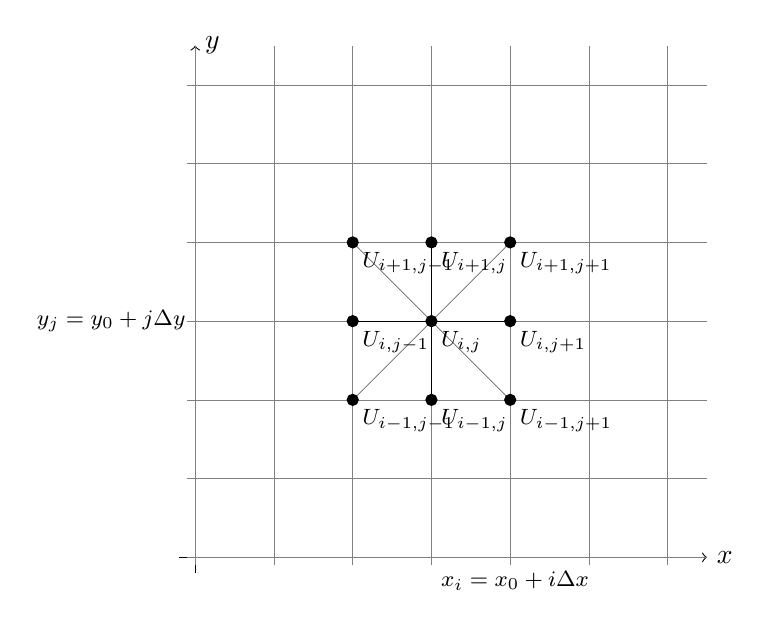
\begin{tikzpicture}
    \draw [->](0,-0.2)--(0,6.5) node[right]{$y$};
    \draw [->](-0.2,0)--(6.5,0) node[right]{$x$};
    \foreach \i in {0,...,6} {
        \draw [very thin,gray] (\i, -0.1) -- (\i,6 + 0.5);
    }
    \foreach \i in {0,...,6} {
        \draw [very thin,gray] (-0.1,\i) -- (6 + 0.5,\i);
    }
    
    \draw (3,-0.3) node[right]{\footnotesize{$x_i = x_0 + i\Delta x$}};
    \draw (0, 3) node[left]{\footnotesize{$y_j = y_0 + j\Delta y$}};
    
    \filldraw[black] (3, 3) circle (2pt) node[anchor=north west] {\footnotesize{$U_{i, j}$}};
    \filldraw[black] (2, 3) circle (2pt) node[anchor=north west] {\footnotesize{$U_{i, j-1}$}};
    \filldraw[black] (4, 3) circle (2pt) node[anchor=north west] {\footnotesize{$U_{i, j+1}$}};
    \filldraw[black] (3, 2) circle (2pt) node[anchor=north west] {\footnotesize{$U_{i-1, j}$}};
    \filldraw[black] (3, 4) circle (2pt) node[anchor=north west] {\footnotesize{$U_{i+1, j}$}};
    \filldraw[black] (4, 4) circle (2pt) node[anchor=north west] {\footnotesize{$U_{i+1, j+1}$}};
    \filldraw[black] (2, 2) circle (2pt) node[anchor=north west] {\footnotesize{$U_{i-1, j-1}$}};
    \filldraw[black] (4, 2) circle (2pt) node[anchor=north west] {\footnotesize{$U_{i-1, j+1}$}};
    \filldraw[black] (2, 4) circle (2pt) node[anchor=north west] {\footnotesize{$U_{i+1, j-1}$}};
    
    \draw [ultra thin] (3, 3) -- (2, 3);
    \draw [ultra thin] (3, 3) -- (4, 3);
    \draw [ultra thin] (3, 3) -- (3, 2);
    \draw [ultra thin] (3, 3) -- (3, 4);
    \draw [ultra thin] (3, 3) -- (4, 4);
    \draw [ultra thin] (3, 3) -- (2, 2);
    \draw [ultra thin] (3, 3) -- (4, 2);
    \draw [ultra thin] (3, 3) -- (2, 4);
    
\end{tikzpicture}
    \caption{Caption}
    \label{fig:stencil+grid}
\end{figure}



\clearpage
%\section{Time Discretization}

\clearpage

%\input{chapters/implementation/imp-signed-dist}
%\section{Updating the Sign Function}
The purpose of the sign function $\sigma(\mathbf{x}, t))$ is to pull the curve in the right direction. As stated, the sign function should be positive when the curve is outside the point set and negative if it is inside of the point set. This may seem like a simple task at first glance, but deciding whether or not the curve should move inwards or outwards is not simple at all.

We first present the strategy that is chosen in our implementation, namely pulling the curve towards its closest points. There is a clear reason behind our choice, but there certainly are drawbacks to the strategy as well, which we will shed light on during this discussion.

The information needed to pull the curve towards the closest point at all times is first of all what parts of space that are closest to which data points and then whether or not that data point is inside or outside of our curve. This is kind of the equivalent but opposite way of looking at the problem, namely whether or not the data points are inside or outside the curve. 


\begin{algorithm}[H]
\SetAlgoLined




\For{$\texttt{contour} \in \texttt{contour\_curves}$}{
    $\texttt{coords}_{t+1} = \texttt{contour}.\texttt{collections.get\_paths().vertices}$ \;
}
\If{$\texttt{shape}(\texttt{coords}_{t+1}) == \texttt{shape}(\texttt{coords}_{t})$}{
    \If{$\|\texttt{coords}_{t+1} - \texttt{coords}_t\|_2 \leq \epsilon$}{
    $\texttt{continue} = \texttt{False}$ \;
    }
}
\KwResult{$\sigma_{n+1}(X, Y)$}
 \caption{Updating $\sigma(\mathbf{x}, t)$}
\label{alg:update-sign}
\end{algorithm}



%%%%%%%%%%%%%%%%%%%%%%%%%%%%%%%%%%%%%%%%%%%%%%%%%%%%%%%%%%%%%%%%%%%
The distance function is local, meaning that it only knows the distance to the closest point and knows nothing about the global arrangement of points. This is the main reason why the sign function is chosen as it is. Remember that it is the distance function which provides the speed and the sign function that decides the direction of the distance-dependent velocity and it is most elegant that the speed and direction is constructed from the same information.

Although it is reasonable, it is not obvious, and there are several reasons why one could want something else. Say that you have noise in your data, and the most obvious curve to draw is one that does not go through any of the points, but passes somewhere in the middle. This kind of behavior would not be encouraged by such a local sign function. 


From the initialization, we saw that the starting curve was chosen to surround all the points in the point set, meaning that the sign function must be positive everywhere. For the behavior of the curve, this means that the distance term is contributing to the speed inwards -- towards the point set. In such cases, where the curve is outside the point set, the sign function has an obvious value. However this is maybe the only situation where this is obvious. 

Say you have noise in your data, and there is no obvious structure in the arrangement of the data points. Then it can be hard to determine whether or not anything is inside or outside of your data points. There could also be situations where the curve is inside and outside simultaneously, if for example again, there are noise and the curve lies somewhere in between data points.

By looking at the data set and the curve, it could be obv

\clearpage

